\documentclass[12pt]{article}
\title{ECE M16 Homework 1}
\usepackage{subcaption}
\author{Lawrence Liu}
\usepackage{graphicx}
\usepackage{amsmath}
\usepackage{placeins}
\newcommand{\Laplace}{\mathscr{L}}
\setlength{\parskip}{\baselineskip}%
\setlength{\parindent}{0pt}%
\usepackage{xcolor}
\usepackage{listings}
\definecolor{backcolour}{rgb}{0.95,0.95,0.92}
\usepackage{amssymb}
\lstdefinestyle{mystyle}{
    backgroundcolor=\color{backcolour}}
\lstset{style=mystyle}

\begin{document}
\maketitle
\section*{Problem 1}
Since there are 26 letters in the English Alphabet, we would need $\lceil \log_2 (26)\rceil=5$ bits to represent this signal.
Therefore we could create a way of encoding the English Alphabet as 5 bits with each letter being encoded as 1+ the encoding of the previous letter, for instance 
A=00000 and B=00001, etc.
\section*{Problem 2}
\subsection*{(a)}
The equation for the circuit is 
$$f(a,b,c)=((a\vee \bar{b})\wedge\bar{c})\vee\overline{((c\wedge\bar{a})\vee b)}$$
Expanding it we get
\begin{align*}
    f(a,b,c)&=((a\wedge\bar{c})\vee (\bar{b}\wedge\bar{c}))
                \vee\overline{((c\wedge\bar{a})\vee b)}\\
    &=((a\wedge\bar{c})\vee (\bar{b}\wedge\bar{c}))
    \vee\overline{((c\vee b)\wedge(\bar{a}\vee b))}\\
    &=((a\wedge\bar{c})\vee (\bar{b}\wedge\bar{c}))
    \vee(\overline{(c\vee b)}\vee\overline{(\bar{a}\vee b)})\\
    &=(a\wedge\bar{c})\vee (\bar{b}\wedge\bar{c})
    \vee(\bar{c}\wedge \bar{b})\vee(a\wedge\bar{b})\\
    &=\boxed{(a\wedge\bar{c})
    \vee(\bar{c}\wedge \bar{b})\vee(a\wedge\bar{b})}
\end{align*}
\subsection*{(b)}
$$\boxed{(a\wedge\bar{c})
\vee(\bar{c}\wedge \bar{b})\vee(a\wedge\bar{b})}$$
\section*{Problem 3}
\subsection*{(a)}
we have $a.\bar{a}=0$, therefore we have
\begin{align*}
    a+0&=a\\
    a+(a.\bar{a})&=a\\
    (a+a).(a+\bar{a})&=a\\
    (a+a).1&=a\\
    a+a&=a
\end{align*}
Likewise we have
\begin{align*}
    a.1&=a\\
    a.(a+\bar{a})&=a\\
    a.a+a.\bar{a}&=a\\
    a.a+0&=a\\
    a.a&=a
\end{align*}
\subsection*{(b)}
From the Boolean Algebra postulates we have: 
$$1.\bar{1}=0$$
Therefore we must have that $\bar{1}=0$
\subsection*{(c)}
Let us consider the case where $\bar{a}$ was not unique, ie for $a_1\neq a_2$, we have
$\bar{a_1}=\bar{a_2}=\bar{a}$. Since $\bar{a}.(a_1+a_2)=0$ and $\bar{a}+(a_1.a_2)=1$, we
have that 
\begin{align*}
    a_1+(\bar{a}.(a_1+a_2))&=a_1\\
    (a_1+\bar{a}).(a_1+a_1+a_2)&=a_1\\
    (a_1+a_2)=a_1
\end{align*}
And that 
\begin{align*}
    a_1.(\bar{a}+(a_1.a_2))&=a_1\\
    (a_1.\bar{a})+(a_1.a_1.a_2)&=a_1\\
    (a_1.a_2)=a_1
\end{align*}
Therefore $a_1=a_2$, and thus $\bar{a}$ must be unique
\section*{Problem 4}
\subsection*{(a)}
\begin{center}
    \begin{tabular}{ |c|c|c||c| }
        p & q & r  & f\\
        \hline
        1 & 1 & 1 & 1\\
        \hline
        1 & 1 & 0 & 1\\
        \hline
        1 & 0 & 1 & 0\\
        \hline
        1 & 0 & 0 & 0\\
        \hline
        0 & 1 & 1 & 1\\
        \hline
        0 & 1 & 0 & 0\\
        \hline
        0 & 0 & 1 & 1\\
        \hline
        0 & 0 & 0 & 0\\
        \hline

    \end{tabular}
\end{center}
\subsection*{(b)}
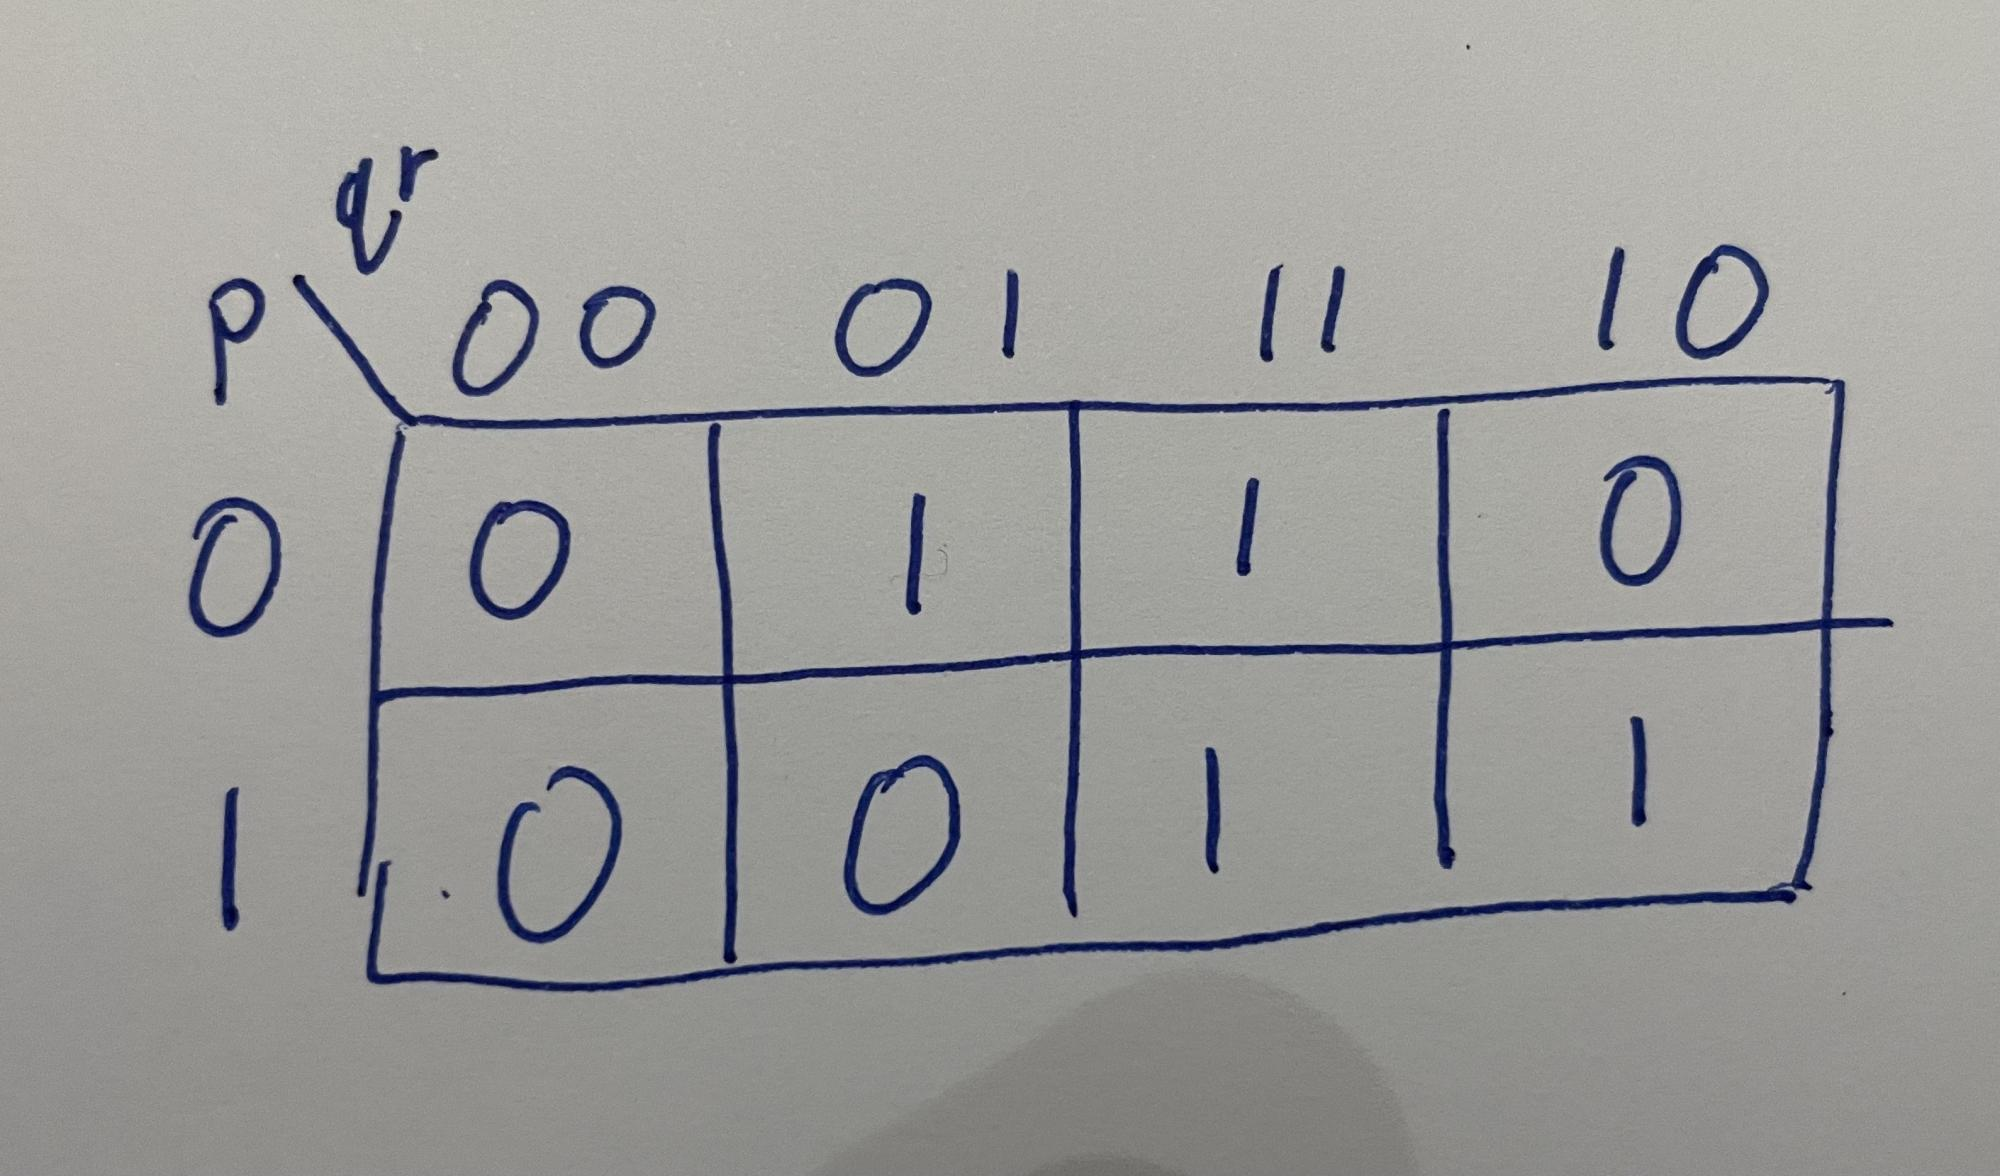
\includegraphics[scale=0.1]{Kmap.jpg}
\subsection*{(c)}
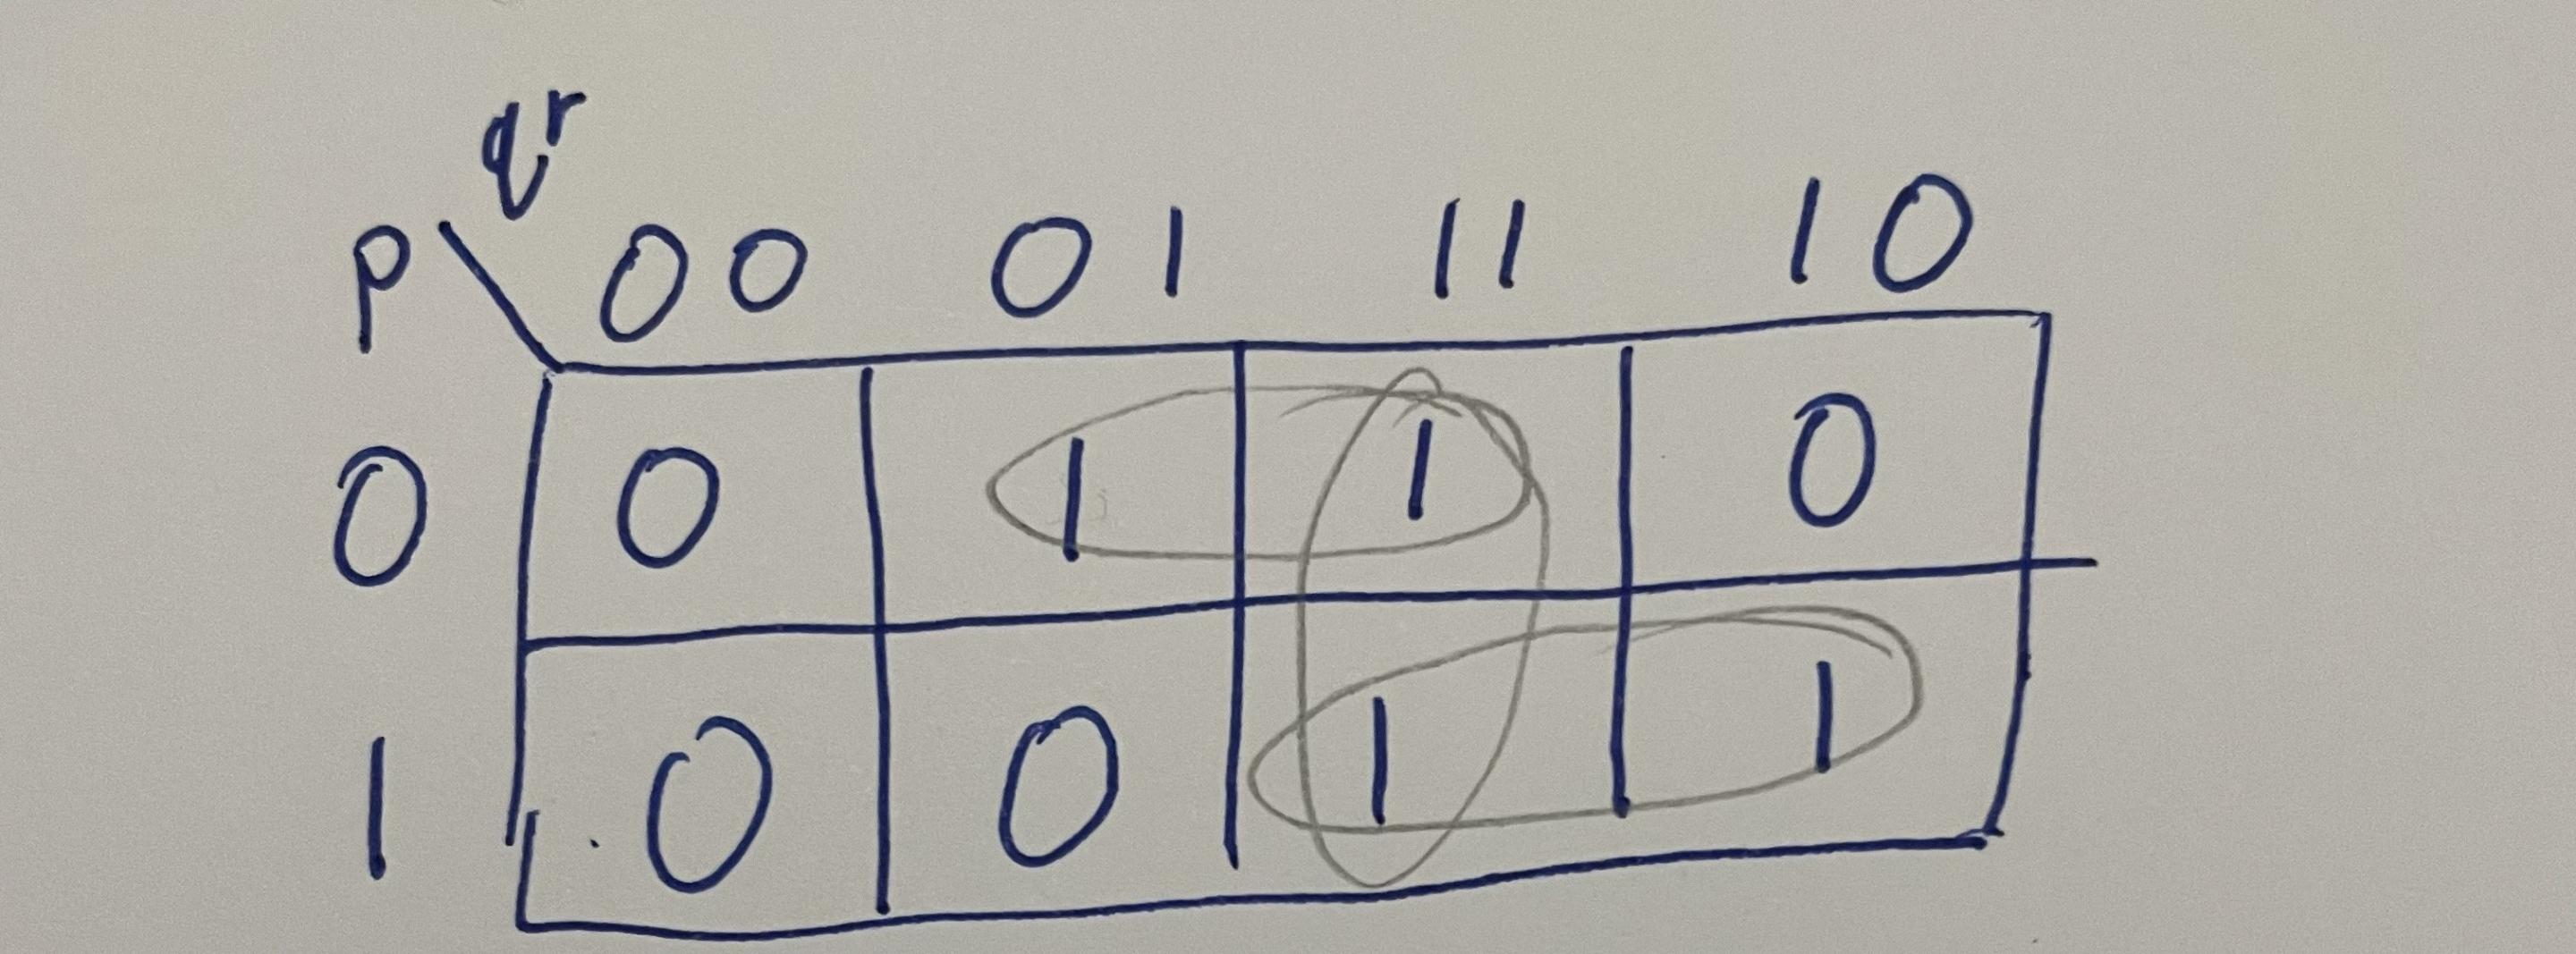
\includegraphics[scale=0.1]{KmapPrime.jpg}
\subsection*{(d)}
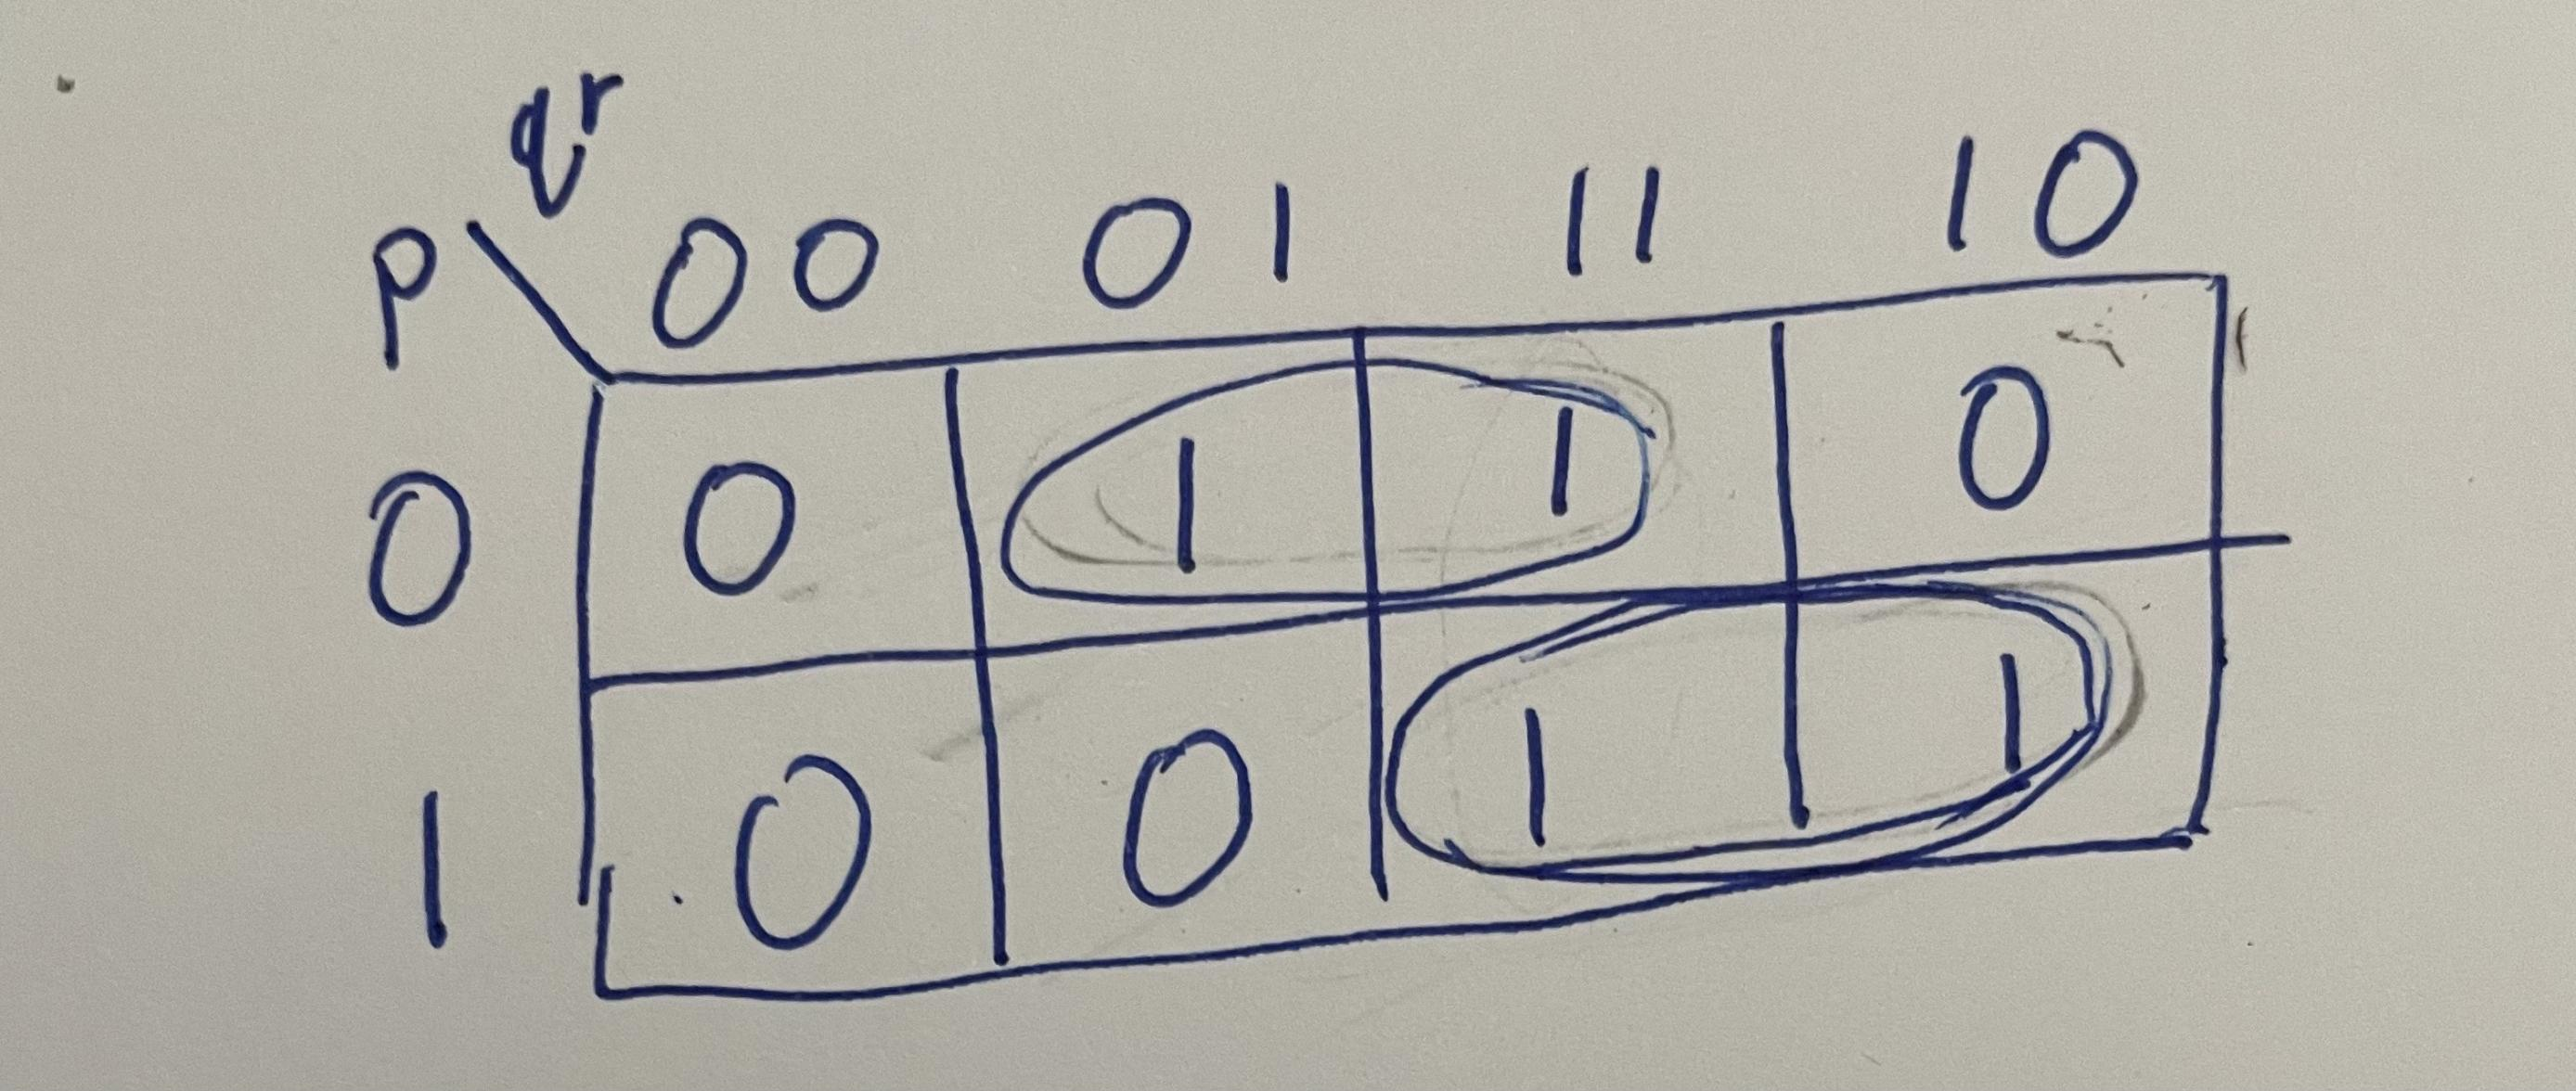
\includegraphics[scale=0.1]{KmapFinal.jpg}
Therefore the boolean expression for the function is 
$$f(p,q,r)=\boxed{(\bar{p}\wedge r)\vee(p\wedge q)}$$
\section*{Problem 5}
\begin{center}
    \begin{tabular}{ |c|c|c||c|c| }
        x & y & z & $\overline{x+y+z}$ & $\overline{x}.\bar{y}.\bar{z}$\\
        \hline
        1 & 1 & 1 & 0 & 0\\
        \hline
        1 & 1 & 0 & 0 & 0\\
        \hline
        1 & 0 & 1 & 0 & 0\\
        \hline
        1 & 0 & 0 & 0 & 0\\
        \hline
        0 & 1 & 1 & 0 & 0\\
        \hline
        0 & 1 & 0 & 0 & 0\\
        \hline
        0 & 0 & 1 & 0 & 0\\
        \hline
        0 & 0 & 0 & 1 & 1\\
        \hline
    \end{tabular}
\end{center}

\begin{center}
    \begin{tabular}{ |c|c|c||c|c| }
        x & y & z & $\overline{x.y.z}$ & $\overline{x}+\bar{y}+\bar{z}$\\
        \hline
        1 & 1 & 1 & 0 & 0\\
        \hline
        1 & 1 & 0 & 1 & 1\\
        \hline
        1 & 0 & 1 & 1 & 1\\
        \hline
        1 & 0 & 0 & 1 & 1\\
        \hline
        0 & 1 & 1 & 1 & 1\\
        \hline
        0 & 1 & 0 & 1 & 1\\
        \hline
        0 & 0 & 1 & 1 & 1\\
        \hline
        0 & 0 & 0 & 1 & 1\\
        \hline
    \end{tabular}
\end{center}
\section*{Problem 6}
\begin{align*}
    (y.\bar{z}+\bar{x}.w).(x.\bar{y}+z.\bar{w})&=y.\bar{z}.(x.\bar{y}+z.\bar{w})+\bar{x}.w.(x.\bar{y}+z.\bar{w})\\
    &=\bar{z}.x.y.\bar{y}+y.\bar{w}.z.\bar{z}+w.\bar{y}.\bar{x}.x+z.\bar{x}.w.\bar{w}
    &=\boxed{0}
\end{align*}
since $x.\bar{x}=y.\bar{y}=w.\bar{w}=z.\bar{z}=0$
\begin{align*}
    (x.y)+(x.(w.z+w.\bar{z}))&=\boxed{(x.y)+(x.w)}
\end{align*}
\end{document}